% Standalone preview of the Results section (article class; IEEEtran not required).
% External theorem/proposition/remark numbers are stubbed to the paper's values so
% cross-references resolve. Compile:  pdflatex results_preview.tex  (twice)
\documentclass[10pt,twocolumn]{article}
\usepackage[letterpaper,margin=0.7in]{geometry}
\usepackage{graphicx,booktabs,amsmath,amssymb}
\usepackage[labelfont=bf]{caption}
\extrafloats{100}
\setcounter{totalnumber}{10}\setcounter{topnumber}{6}
\renewcommand{\topfraction}{.95}\renewcommand{\floatpagefraction}{.85}
\renewcommand{\textfraction}{.05}
\makeatletter
\def\stub#1#2{\global\@namedef{r@#1}{{#2}{1}}}
\stub{thm:params}{2}\stub{thm:validity}{9}
\stub{prop:soft}{11}\stub{prop:buffer}{12}\stub{prop:est}{10}
\stub{rem:gap}{1}\stub{rem:rho}{14}\stub{rem:eps}{17}\stub{rem:buffer}{16}
\stub{asm:robot}{2}
\stub{sec:variants}{VII}\stub{sec:adversary}{V}\stub{sec:estimation}{VI}
\stub{eq:bicycle}{9}
\newcommand{\citestub}[2][\@empty]{\ifx\@empty#1[1]\else[1, #1]\fi}\let\cite\citestub
\makeatother
% graphics live in ../results
\graphicspath{{../results/}}
\title{\vspace{-2.5em}\textbf{AR-DPCBF --- Results Section (compiled preview)}}
\date{}
\begin{document}
\maketitle
% =====================================================================
%  Section VIII -- SIMULATION STUDY  (AR-DPCBF)
%  Reorganised to tell a coherent argument:
%    Setup -> Problem & Fix -> Generality -> Cost -> Theory -> Summary
%  Figures are vector PDFs (Illustrator-editable).
%  Requires: \usepackage{graphicx,booktabs,amsmath,amssymb}
% =====================================================================
\section{Simulation Study}
\label{sec:results}

We present the study as a single argument rather than a catalogue of
experiments. After fixing the platform, scenario, and metrics
(Section~\ref{sec:setup}), we establish the central claim---that the
constant-velocity assumption makes DPCBF fail \emph{silently} under
maneuvering obstacles, and that the adversarial variants remove the
failure---quantitatively and with a paired significance test, then
illustrate it on representative trajectories (Section~\ref{sec:core}). We
next ask how general the result is along the two independent axes of the
threat space, adversary capability and scene density, the latter being where
the soft variants justify their existence through
Propositions~\ref{prop:soft}--\ref{prop:buffer}
(Section~\ref{sec:generality}). Having established robustness, we quantify
its price and the single parameter that tunes it (Section~\ref{sec:price}).
Finally we validate the three theoretical guarantees directly---the validity
condition of Theorem~\ref{thm:validity}, fail-safe behavior under capability
misspecification, and the online estimator of Proposition~\ref{prop:est}
(Section~\ref{sec:theory})---before concluding (Section~\ref{sec:summary}).

% ---------------------------------------------------------------------
\subsection{Experimental Setup}
\label{sec:setup}

\paragraph{Platform and parameters}
The robot is the kinematic bicycle~\eqref{eq:bicycle} with the parameters
of~\cite[Table~I]{park2026dpcbf}: rear-axle length $\ell_r=0.20$\,m,
acceleration limit $a_{\max}=5.0$\,m\,s$^{-2}$, slip-angle limit
$\beta_{\max}=0.28$\,rad, speed range $v\in[v_{\min},v_{\max}]$ with
$v_{\max}=3.5$\,m\,s$^{-1}$ and cruise reference $v_{\mathrm{des}}=2.5$\,
m\,s$^{-1}$, combined safety radius $r=1.0$\,m, sensing radius $15$\,m, and
barrier gains $k_\lambda=0.144$, $k_\mu=0.505$. Two settings are dictated by
the adversarial extension and are stated explicitly for reproducibility: the
minimum speed is raised to $v_{\min}=1.0$\,m\,s$^{-1}$
(Assumption~\ref{asm:robot}: steering authority scales as $v^2/\ell_r$ and
vanishes at rest, so a positive floor is required to defend the barrier; this
yields $c_{\min}=\min\{a_{\max},v_{\min}^2\beta_{\max}/\ell_r\}=1.40$), and
the pre-emption gain is $\gamma=3.0$ unless swept. The penalty weight is
$\rho=10.0$ and the buffer width $\varepsilon=0.3$
(Remarks~\ref{rem:rho}--\ref{rem:eps}).

\paragraph{Scenario family}
The robot navigates from $(2,12)$ to a goal at $x=50$\,m through a field of
$N$ obstacles, of which $n_{\mathrm{adv}}$ are adversarial. Crucially, the
adversarial set is \emph{not} chosen at random: the $n_{\mathrm{adv}}$
obstacles \emph{closest to the robot's start} are designated as maneuvering
adversaries, since these are the agents that genuinely threaten the robot;
the remainder are benign constant-velocity movers consistent with the DPCBF
modeling assumption. Each adversary executes the worst-case
capability-saturating maneuver of Section~\ref{sec:adversary} that minimizes
the robot's barrier rate $\dot h$. The representative operating point used
throughout (unless a quantity is being swept) is $N=10$, $n_{\mathrm{adv}}=5$,
and capability $\kappa=0.98$\,m\,s$^{-2}$ (split as
$a_{\mathrm{obs,max}}=0.5$, $\omega_{\mathrm{obs,max}}=0.4$,
$v_{\mathrm{obs,nom}}=1.2$), comfortably inside the validity envelope
$\kappa<c_{\min}=1.40$. Episodes integrate at $\Delta t=0.06$\,s with an RK4
step and a $40$\,s horizon.

\paragraph{Metrics}
We separate three distinct safety axes that are often conflated.
\emph{Barrier violation} is the event $\min_t h(x(t))<0$, i.e. the robot left
the nominal DPCBF safe set---this is the primary metric because it is exactly
the silent-failure event of Remark~\ref{rem:gap}, detectable even when no
collision occurs. \emph{Collision} is the geometric event $d(t)<r$.
\emph{QP infeasibility} is the per-cycle rate at which a controller's safety
program admits no input. We additionally report \emph{success} (goal reached
and collision-free), path length, time-to-goal, and QP cost
$\sum_t\lVert u-u_{\mathrm{ref}}\rVert^2$. Unless noted, each condition
aggregates $n=40$ independent seeds, and uncertainty is reported as $95\%$
bootstrap confidence intervals (CIs, $4000$ resamples). Paired method
comparisons use the exact two-sided McNemar test on common seeds.

% =====================================================================
\subsection{The Silent-Failure Mode and Its Removal}
\label{sec:core}

We begin by demonstrating that the proposed controllers do what they are
designed to do---navigate a dense field of maneuvering adversaries without
breaching the safety certificate---and then establish the effect
quantitatively with a controlled sweep and a paired significance test.

\paragraph{Qualitative navigation}
Figs.~\ref{fig:tl_soft}--\ref{fig:tl_buf} show two representative
trajectories of the proposed controllers at the representative condition
($N=10$, $n_{\mathrm{adv}}=5$). Under the nearest-adversary scenario the
adversaries (red) begin clustered around the robot's start while the benign
movers (gray) lie toward the goal. The Soft controller
(Fig.~\ref{fig:tl_soft}) lifts over the adversary wall and threads the pack,
reaching the goal at $22.0$\,s with $\min_t h=+0.32$: the nominal barrier is
never violated. For the Buffer controller (Fig.~\ref{fig:tl_buf}) we
additionally render the position-space unsafe sets exactly: the set $\{h<0\}$
is a closed parabolic lobe in the line-of-sight frame---bounded, not the
unbounded cone of a velocity-obstacle method---and the adversarial set
$\{h^*<0\}$ is the uniformly wider lobe whose gap is the adversarial widening
of Theorem~\ref{thm:params}. Buffer keeps the robot outside even the
\emph{contracted} set throughout, $\min_t h^*=+0.21>0$, in contrast to the
Soft trajectory which grazes it ($\min_t h^*=-0.06$); this is the proactive
advantage of Remark~\ref{rem:buffer} made visible. These trajectories show
the controllers operating exactly as intended; the remainder of this section
quantifies, across difficulty and with statistical rigor, the failure they
prevent.

\begin{figure*}[t]
  \centering
  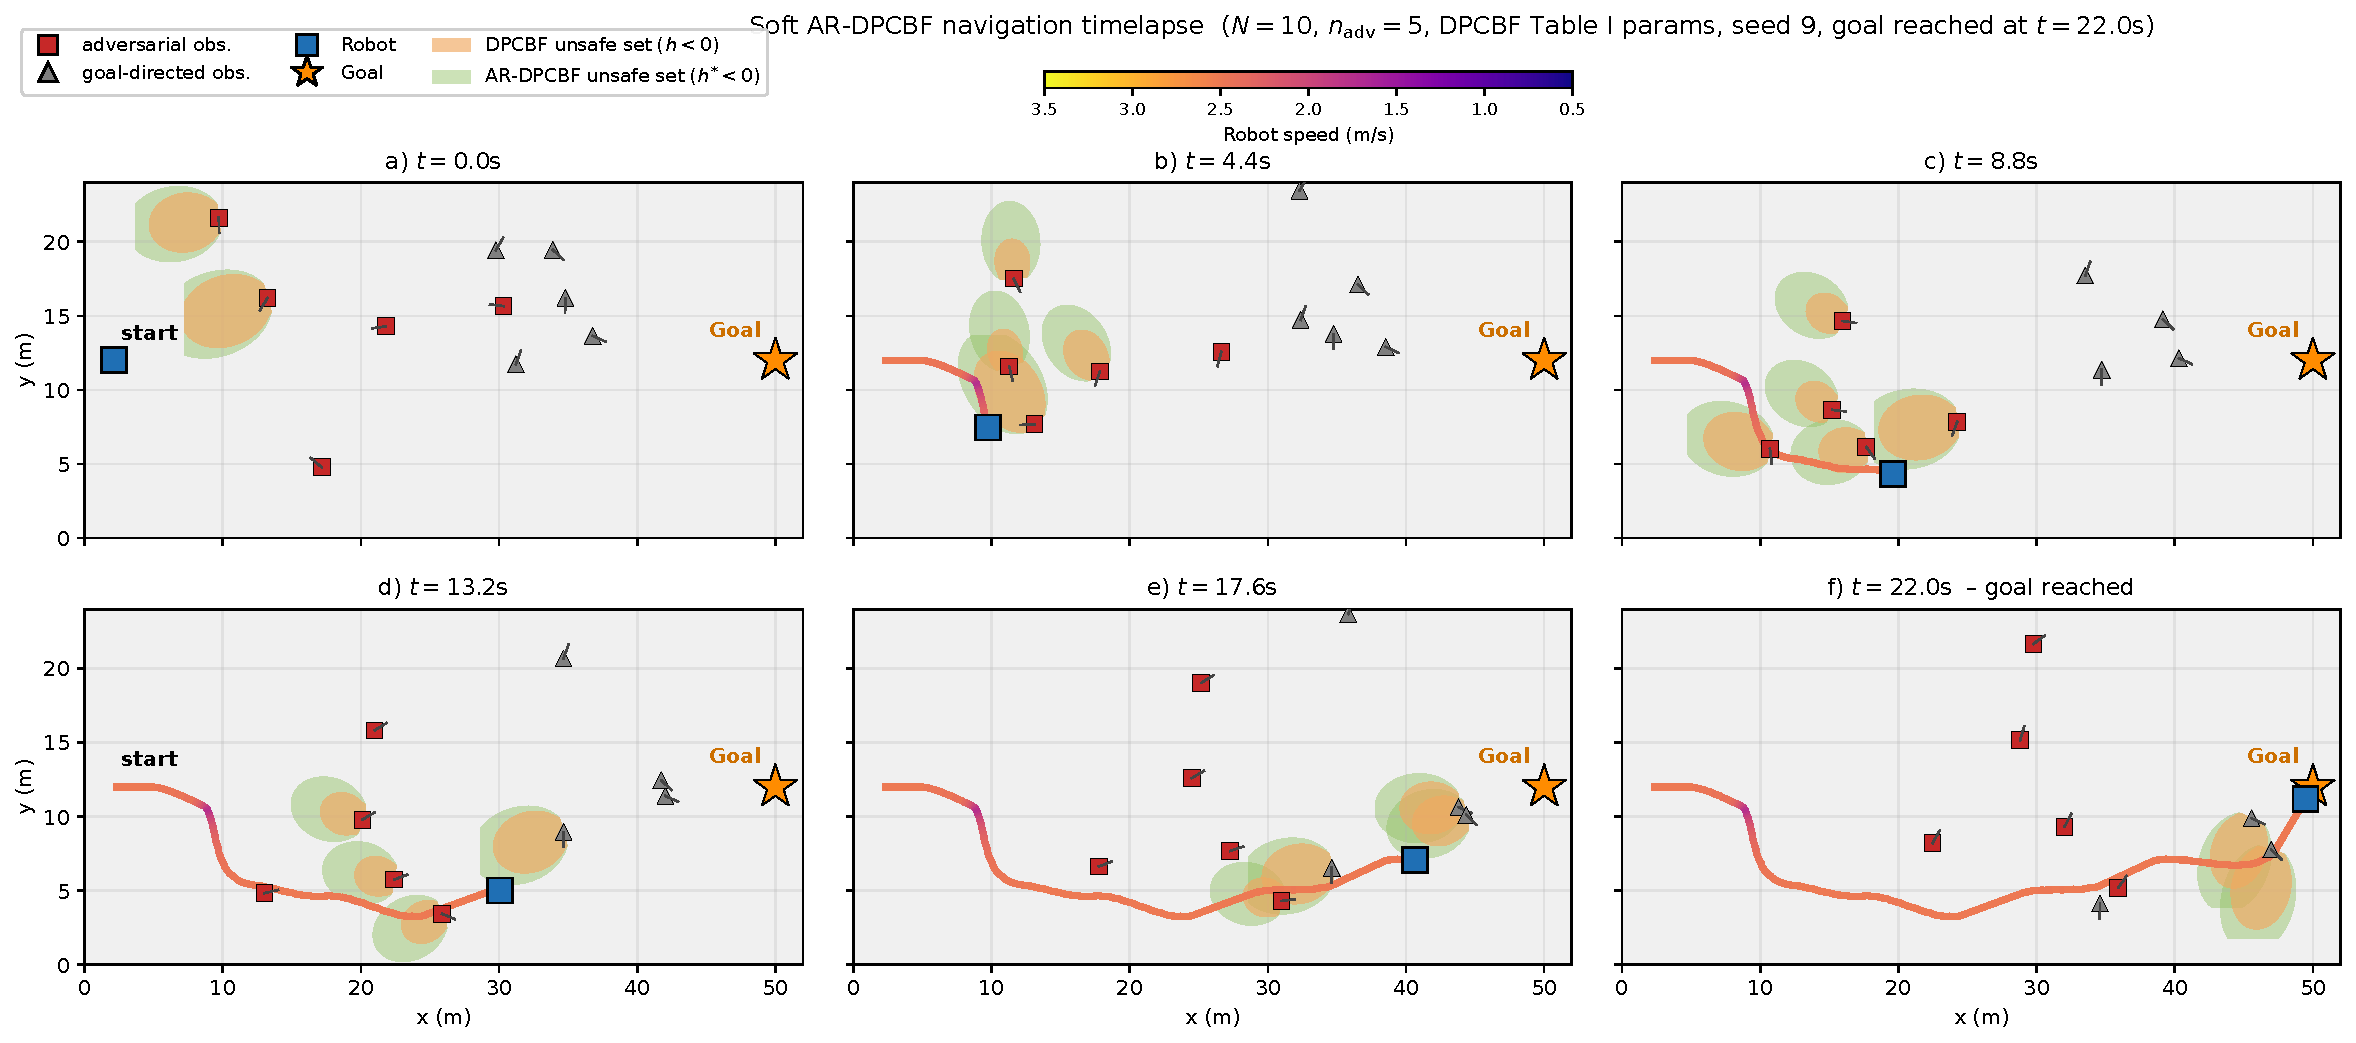
\includegraphics[width=\textwidth]{fig_timelapse_fix.pdf}
  \caption{Soft AR-DPCBF navigation timelapse ($N=10$, $n_{\mathrm{adv}}=5$,
  nearest-adversary, seed~9; goal reached at $22.0$\,s, $\min_t h=+0.32$).
  Orange: $\{h<0\}$; green: $\{h^*<0\}$.}
  \label{fig:tl_soft}
\end{figure*}

\begin{figure*}[t]
  \centering
  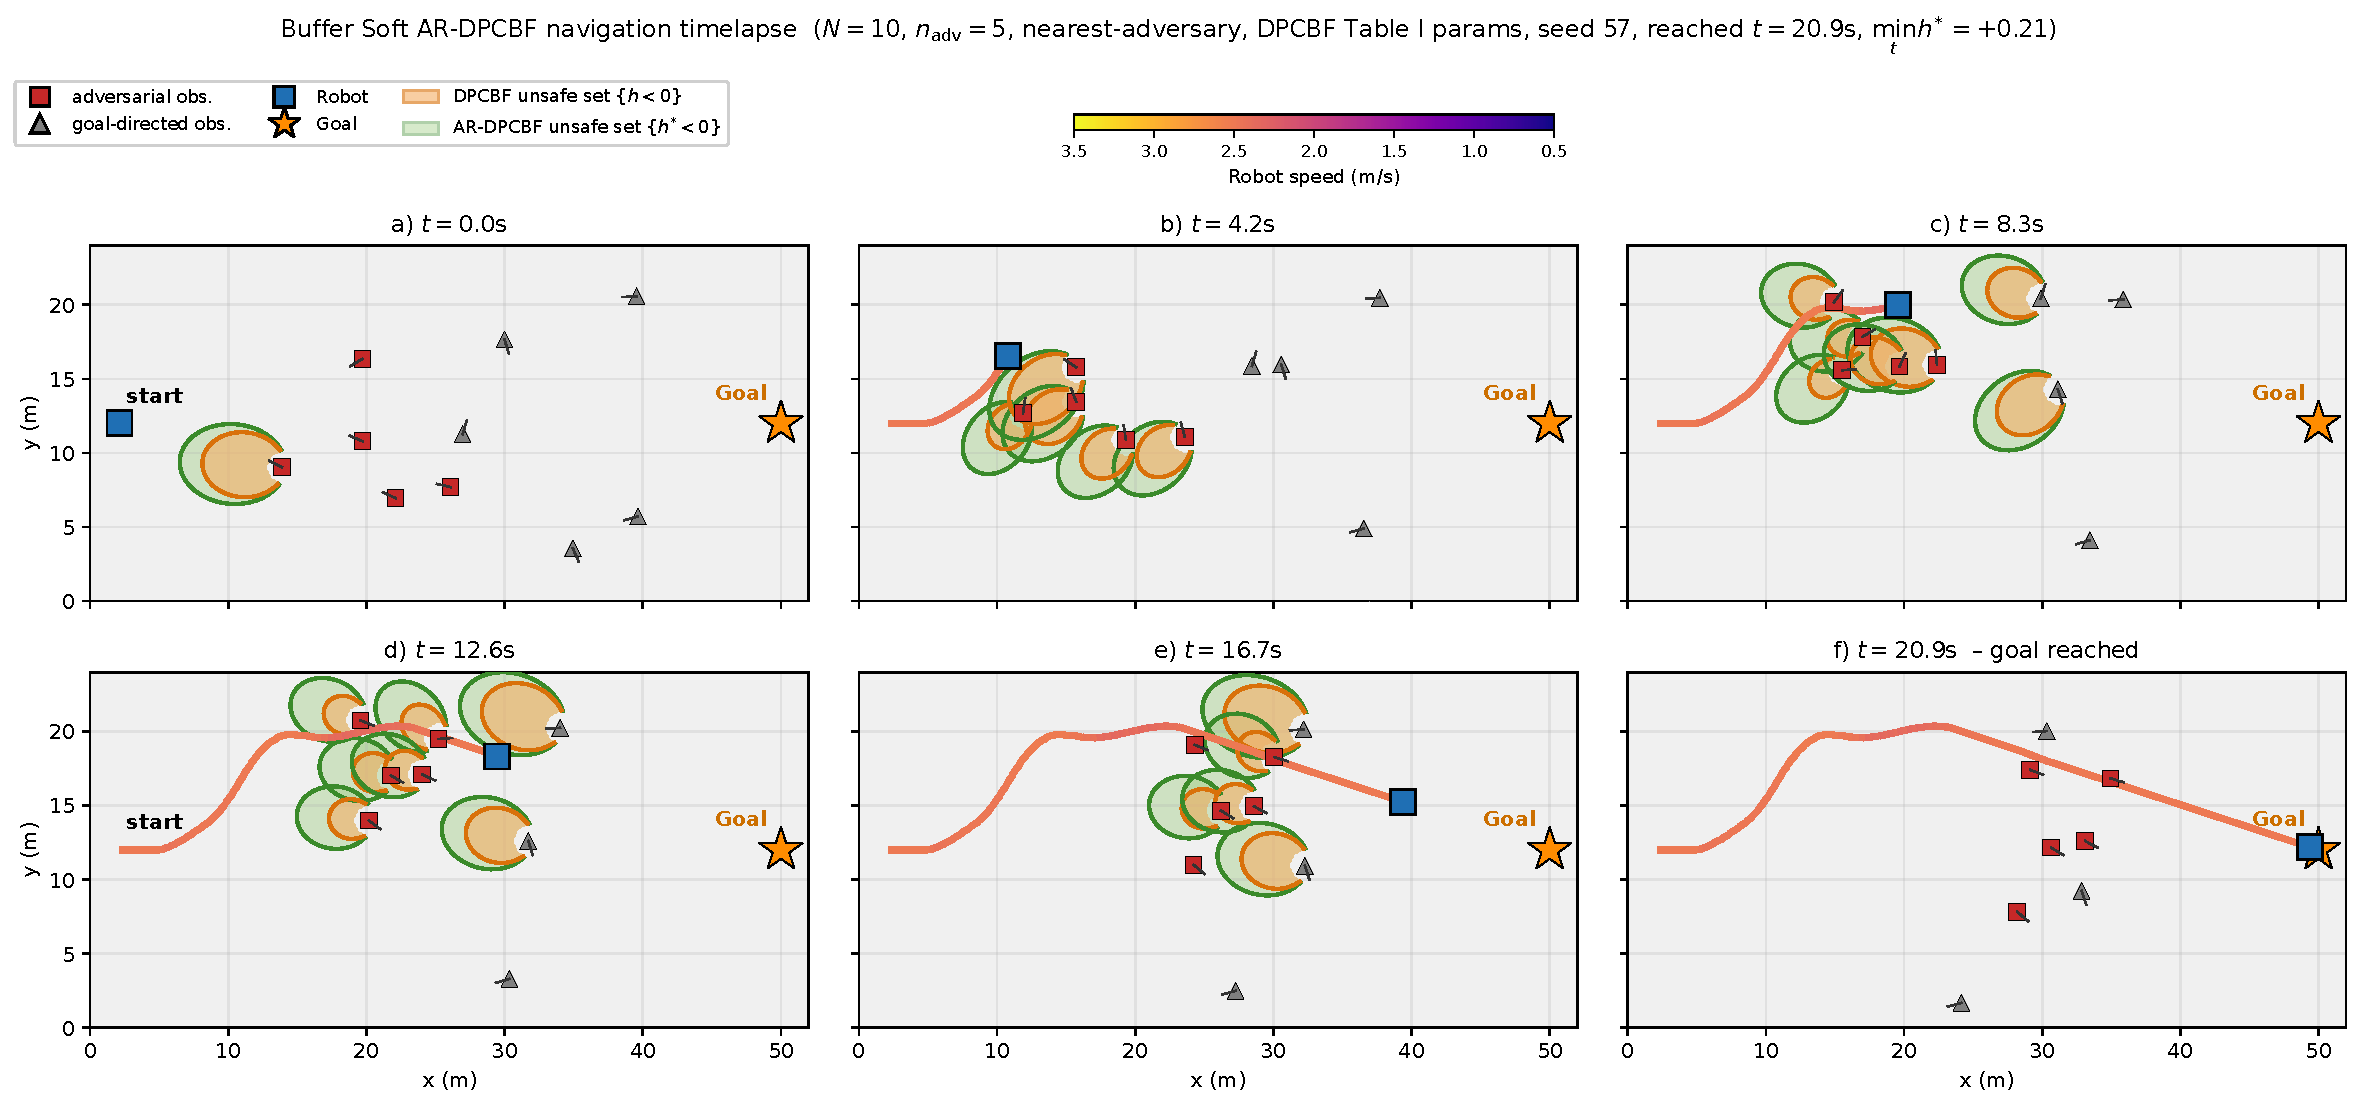
\includegraphics[width=\textwidth]{fig_timelapse_buf.pdf}
  \caption{Buffer Soft AR-DPCBF navigation timelapse (seed~57,
  $\min_t h^*=+0.21$). The unsafe sets are drawn with their exact $\{h=0\}$
  (orange) and $\{h^*=0\}$ (green) boundaries; the green set is the uniformly
  wider adversarial widening. The proactive buffer keeps the robot outside
  the contracted set throughout.}
  \label{fig:tl_buf}
\end{figure*}

\paragraph{Adversary count}
The trajectories above are illustrative; to measure the effect across
difficulty rather than on single seeds, Fig.~\ref{fig:adv} sweeps the number
of adversaries $n_{\mathrm{adv}}\in\{0,\dots,15\}$ at a dense fixed population
$N=15$, so that the failure is exercised all the way to the all-adversarial
limit. At $n_{\mathrm{adv}}=0$ (all obstacles benign, constant velocity) every
method is identical and safe: the recovery property of
Theorem~\ref{thm:params}(ii) holds and the adversarial barrier collapses to
the nominal one. As soon as obstacles maneuver, the silent failure predicted
by Remark~\ref{rem:gap} appears, and we read it \emph{first on the
barrier-violation axis}, because that is precisely the event the QP fails to
detect. With a single adversary DPCBF already violates the certificate in
$35\%$ of trials; this rises to $72\%$ at $n_{\mathrm{adv}}=3$, holds a
plateau near $80\%$ through the mid-range, and reaches $95\%$ when every
obstacle is adversarial. The collision rate is the downstream consequence and
is correspondingly lower and noisier---growing from $30\%$ to $60\%$ over the
same range---because the robot, being faster than the obstacles, frequently
outruns an encounter even after the certificate has been breached. This very
gap between an $80$--$95\%$ violation rate and a $30$--$60\%$ collision rate
is itself the sharpest evidence of the \emph{silent} nature of the failure:
the safety certificate is breached far more often than contact actually
occurs, exactly the regime that motivates a detector at the certificate
level. All three AR variants suppress both axes across the entire range.
Buffer Soft AR-DPCBF is the strongest, holding violations to $17$--$30\%$ and
collisions to $5$--$25\%$; Soft is intermediate; and Hard, despite enforcing
the contracted barrier, is limited by the feasibility losses of
Section~\ref{sec:generality} (violations rising to $65\%$ at the
all-adversarial extreme). The ordering
$\text{Buffer}<\text{Soft}<\text{Hard}<\text{DPCBF}$ in violation holds
throughout, the DPCBF confidence band separates from every AR variant for
$n_{\mathrm{adv}}\ge 3$, and across all AR variants the collision rate is
reduced by a factor of $3$--$5\times$ relative to the unprotected baseline.

\begin{figure*}[t]
  \centering
  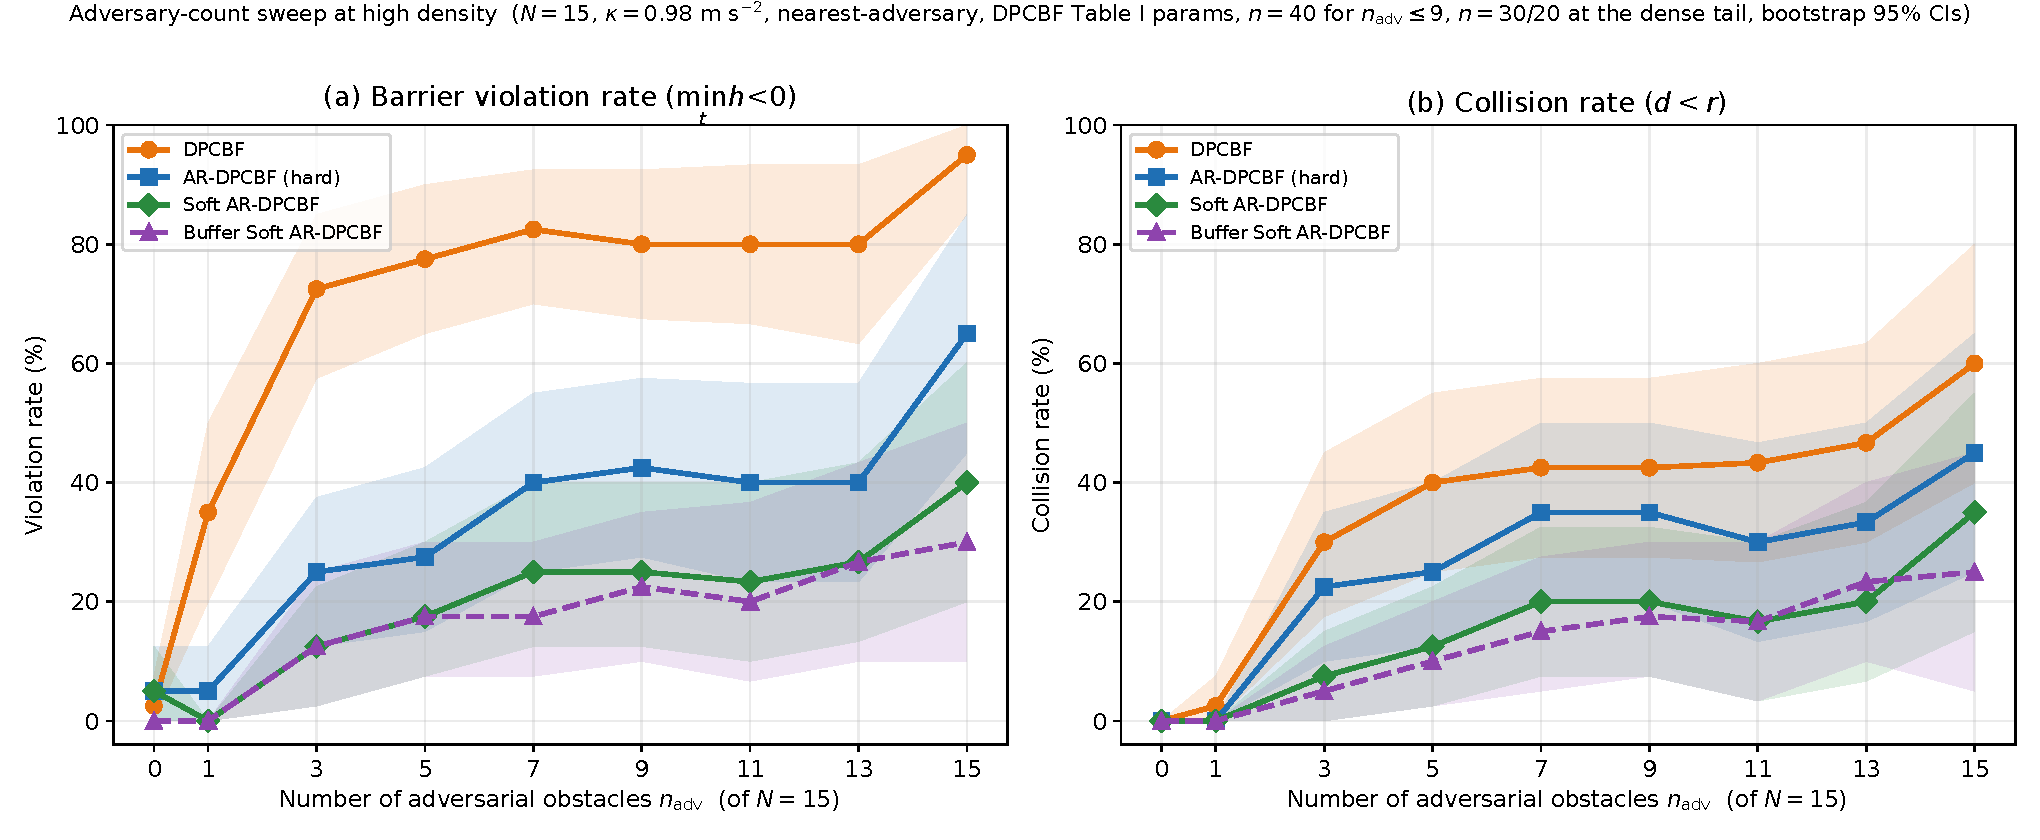
\includegraphics[width=\textwidth]{fig_sweep15_ci_fix.pdf}
  \caption{Safety versus number of adversaries at high density
  ($N=15$, $\kappa=0.98$; $n=40$ for $n_{\mathrm{adv}}\le 9$ and reduced at
  the dense tail; $95\%$ bootstrap CIs). (a)~Barrier-violation rate
  $P[\min_t h<0]$---the silent-failure metric---which DPCBF drives to $95\%$
  while the AR variants remain low; (b)~collision rate, the downstream
  consequence, reaching $60\%$ for DPCBF at the all-adversarial limit. All
  methods coincide at $n_{\mathrm{adv}}=0$ (recovery). The large
  violation--collision gap is the signature of the silent failure.}
  \label{fig:adv}
\end{figure*}

\paragraph{Statistical significance}
To confirm these differences are not sampling artifacts we run a paired
protocol over six dense conditions ($N=15$,
$n_{\mathrm{adv}}\in\{5,7,9,11,13,15\}$, $120$ paired trials) and apply the
exact McNemar test (Fig.~\ref{fig:mcnemar}). Pooled collision rates are
DPCBF $49\%\!\to$ Hard $35\%\!\to$ Soft $24\%\!\to$ Buffer $21\%$, and pooled
violation rates $84\%\!\to46\%\!\to29\%\!\to25\%$. Buffer Soft AR-DPCBF is the
only method that significantly improves on \emph{both} DPCBF and Hard AR on
\emph{both} axes: versus DPCBF the collision discordant counts are
$(b_{10},b_{01})=(35,1)$, $p<10^{-3}$; versus Hard, $(20,3)$,
$p=5\times10^{-4}$. The DPCBF$\to$Hard reduction is itself significant
($p=10^{-4}$), confirming that even the hard certificate removes collisions
relative to the baseline once the threat is co-located with the robot. The
Hard$\to$Soft collision improvement is only marginal ($p=0.011$), so we do
not over-claim a soft-over-hard advantage on collisions; on violations every
pairwise comparison is significant at $p<10^{-3}$. Per-condition discordant
counts are small ($n=20$), so the $p<10^{-3}$ results are pooled; isolating
significance within each condition would require $n\!\approx\!50$--$60$.

\begin{figure*}[t]
  \centering
  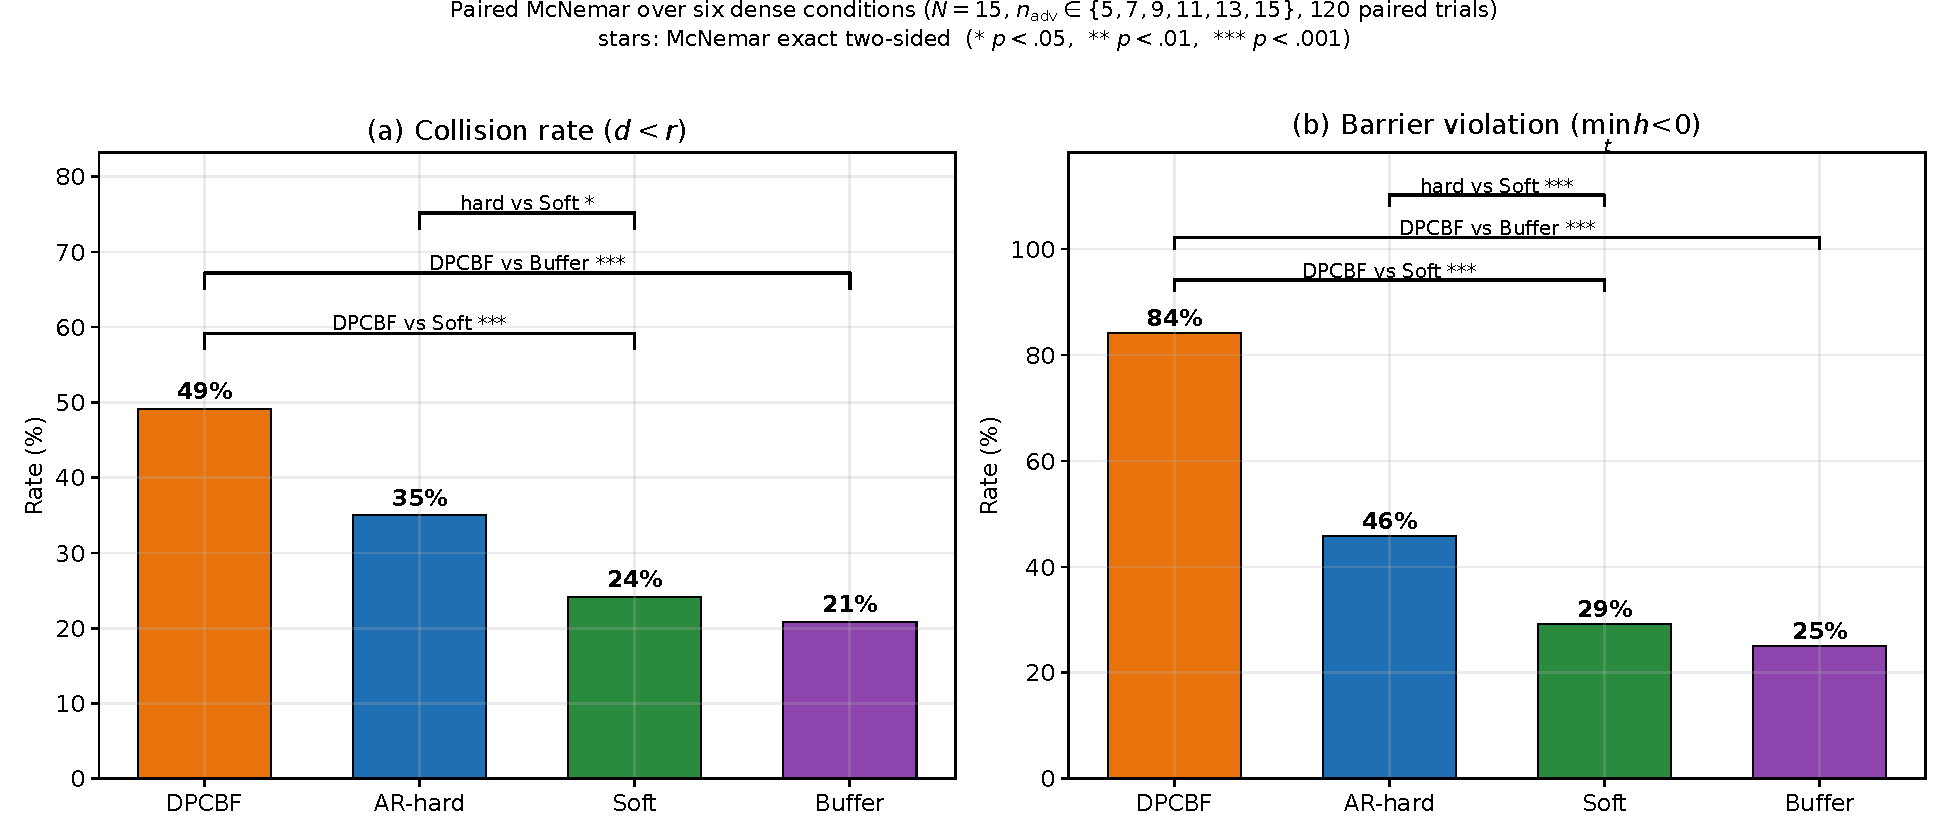
\includegraphics[width=\textwidth]{fig_mcnemar15_fix.pdf}
  \caption{Paired McNemar comparison over six dense conditions
  ($N=15$, $120$ paired trials). (a)~Collision and (b)~violation rates with
  significance brackets ($^{*}p<.05$, $^{**}p<.01$, $^{***}p<.001$). Buffer
  Soft AR-DPCBF dominates both baselines on both axes.}
  \label{fig:mcnemar}
\end{figure*}

% =====================================================================
\subsection{Generality Across the Threat Space}
\label{sec:generality}

The preceding section fixed the population and varied the adversarial
\emph{fraction}. We now vary the two underlying axes of the threat space
independently: the \emph{capability} of each adversary, and the total
\emph{density} of the scene. The first establishes that the result is not an
artifact of one capability value; the second is where the soft variants earn
their place.

\paragraph{Adversary capability}
Fig.~\ref{fig:cap} fixes $n_{\mathrm{adv}}=5$ and sweeps the per-obstacle
capability $\kappa$ from $0$ to $c_{\min}=1.4$. At $\kappa=0$ all four
controllers collapse onto a common $\sim\!10\%$ value
(Theorem~\ref{thm:params}(ii), recovery), confirming that AR-DPCBF adds
robustness continuously and with no penalty when the obstacle cannot
maneuver. For $\kappa>0$ the DPCBF violation band immediately detaches,
peaking at $92\%$ near $\kappa=0.4$ before declining---a non-monotonicity
explained by the fact that very aggressive adversaries overshoot the
slower-reacting baseline. Throughout, all three AR variants form a tight
low-violation cluster well separated from DPCBF, with Buffer lowest
($12\%$--$28\%$). The figure marks the validity edge $\kappa=c_{\min}$: the
guarantee of Theorem~\ref{thm:validity} applies to its left, and the AR
variants remain controlled up to and slightly beyond it, with the graceful
degradation past the edge quantified in Section~\ref{sec:theory}.

\begin{figure}[t]
  \centering
  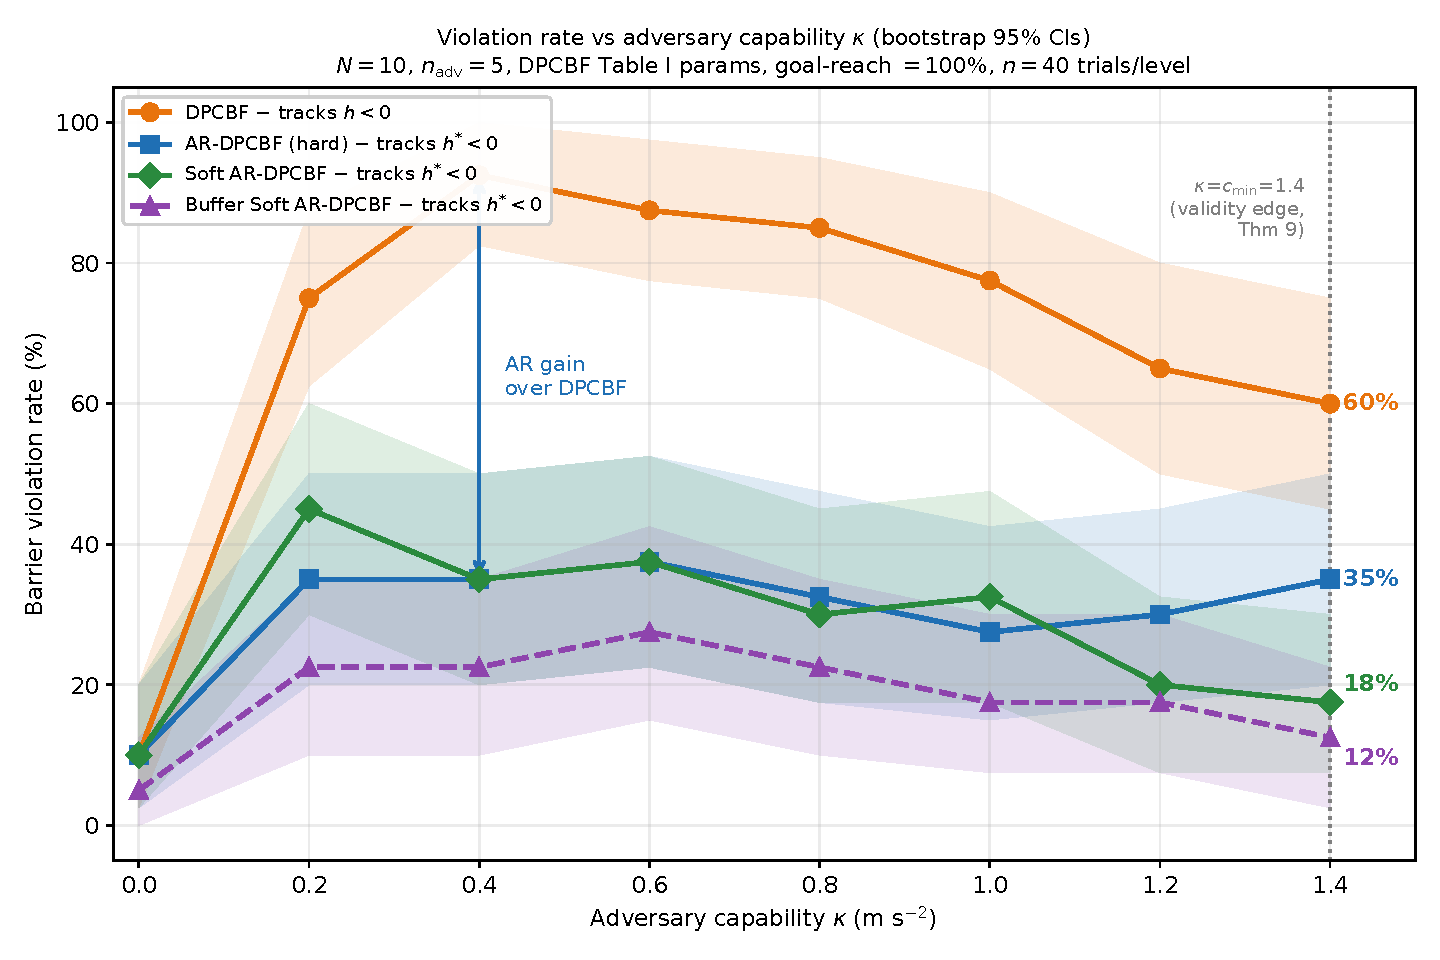
\includegraphics[width=\columnwidth]{fig_kappa10_ci_fix.pdf}
  \caption{Barrier-violation rate versus adversary capability $\kappa$
  ($N=10$, $n_{\mathrm{adv}}=5$, $n=40$). All methods coincide at $\kappa=0$
  (recovery); DPCBF detaches sharply while AR variants remain low. The dotted
  line marks the validity edge $\kappa=c_{\min}=1.40$.}
  \label{fig:cap}
\end{figure}

\paragraph{Density and feasibility}
Whereas the capability sweep stresses the \emph{strength} of adversaries, the
density sweep stresses the \emph{clutter} of the scene, holding the
adversarial fraction at one half and varying $N$ from $1$ to $30$. This is
the experiment that the soft variants exist for: their defining property
(Propositions~\ref{prop:soft}--\ref{prop:buffer}) is that they keep the DPCBF
constraint hard and therefore inherit its feasibility, whereas the Hard
variant enforces the contracted barrier and can lose it.
Fig.~\ref{fig:density}(a) confirms this directly: the Hard-AR QP-infeasibility
rate climbs monotonically with $N$ to $\approx 4.9\%$, while Soft
($\approx 0.8\%$) and Buffer ($\approx 0.3\%$) stay essentially flat near
zero. Two points are worth making precisely. First, the soft variants'
infeasibility is not merely \emph{equal} to DPCBF's but \emph{below} it
($\approx 2.2\%$ at $N=30$): Propositions~\ref{prop:soft}--\ref{prop:buffer}
guarantee equality of the feasible \emph{set at a given state}, not of the
trajectory-aggregate rate, and because the soft penalties proactively steer
away from tight pockets they simply \emph{visit} near-infeasible
configurations less often. Second, the success-rate panel
(Fig.~\ref{fig:density}(b))---the \emph{liveness} consequence of feasibility,
folding in goal-reaching as well as collision-avoidance---orders the methods
$\text{Buffer}>\text{Soft}>\text{Hard}>\text{DPCBF}$ at every density, with
DPCBF collapsing to $50\%$ (feasible but colliding) and Buffer holding
$\approx 86\%$ at $N=30$. The success CIs are wide at $n=20$ and overlap, so
we present the infeasibility panel as the primary evidence for
Propositions~\ref{prop:soft}--\ref{prop:buffer} and the success panel as
corroborating. Note that this sweep is complementary to, not a repetition of,
Fig.~\ref{fig:adv}: the former varies total clutter at fixed composition and
reports feasibility/liveness, the latter varies composition at fixed clutter
and reports safety.

\begin{figure*}[t]
  \centering
  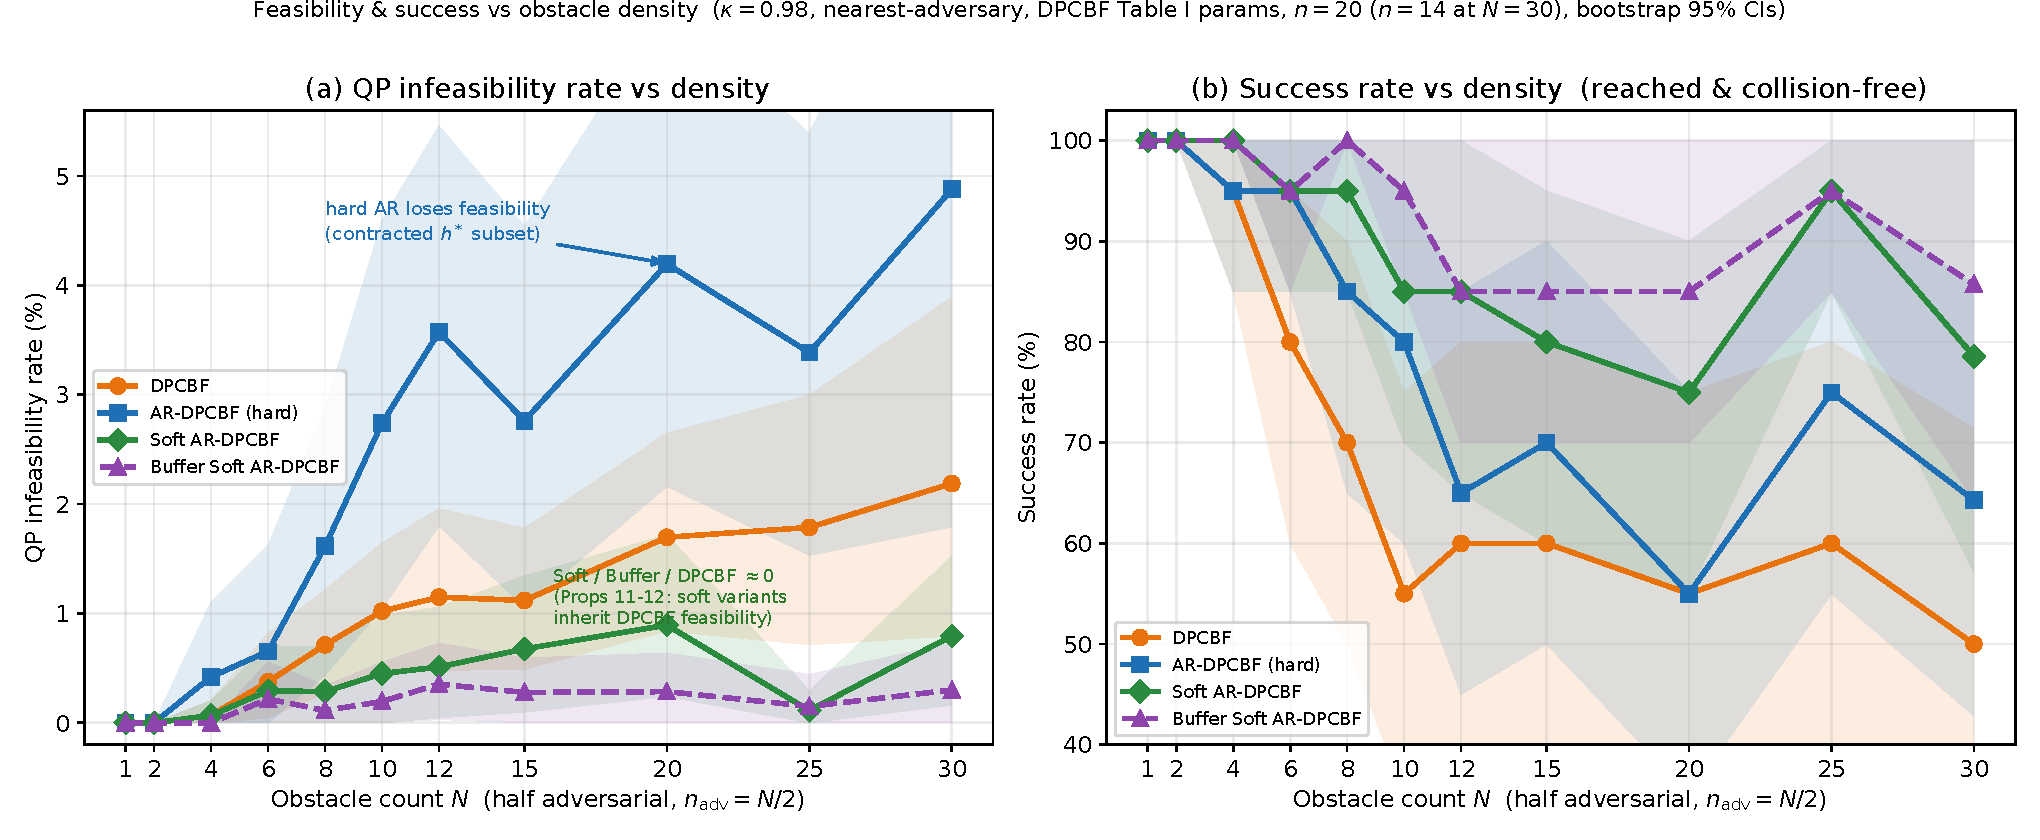
\includegraphics[width=\textwidth]{fig_density.pdf}
  \caption{Feasibility and liveness versus obstacle density $N$ (half
  adversarial, $\kappa=0.98$). (a)~QP-infeasibility rate: Hard-AR diverges
  while Soft/Buffer remain near zero, the empirical signature of
  Propositions~\ref{prop:soft}--\ref{prop:buffer}; (b)~success rate (reached
  and collision-free).}
  \label{fig:density}
\end{figure*}

% =====================================================================
\subsection{The Price of Robustness and Its Tuning}
\label{sec:price}

Robustness is not free. Having established that the AR variants are safer and
remain feasible, we now quantify what they cost and expose the single design
parameter that trades cost against safety.

\paragraph{Cost of robustness}
Fig.~\ref{fig:cost} reports the cost at the representative condition. The
spatial cost is small and monotonic in how proactive the method is: path
length grows $50.1\!\to\!51.4\!\to\!52.3\!\to\!53.6$\,m
(DPCBF$\to$Hard$\to$Soft$\to$Buffer, a $7\%$ increase for Buffer) and
time-to-goal $20.6\!\to\!21.8$\,s ($6\%$), with collisions simultaneously
falling from $42\%$ to $8\%$. The control-effort cost, however, does
\emph{not} follow the naive expectation that the unconstrained baseline is
cheapest. The QP-cost distribution is heavy-tailed and is therefore reported
as a median with a logarithmic box plot, following the convention
of~\cite{park2026dpcbf}. On the median, DPCBF is the \emph{most} effortful
($78$), not the least, because under a maneuvering adversary it reacts late
and violently and the squared cost penalizes those spikes; the soft penalties
produce smoother control (Soft $22$, Buffer $47$). In other words, the cost
of robustness is paid in a modest path/time detour, while control effort
actually \emph{decreases}---a consequence of replacing DPCBF's reactive
evasions with proactive steering. Hard AR is the poorest trade, combining
high control effort with the feasibility losses of Section~\ref{sec:generality}.

\begin{figure*}[t]
  \centering
  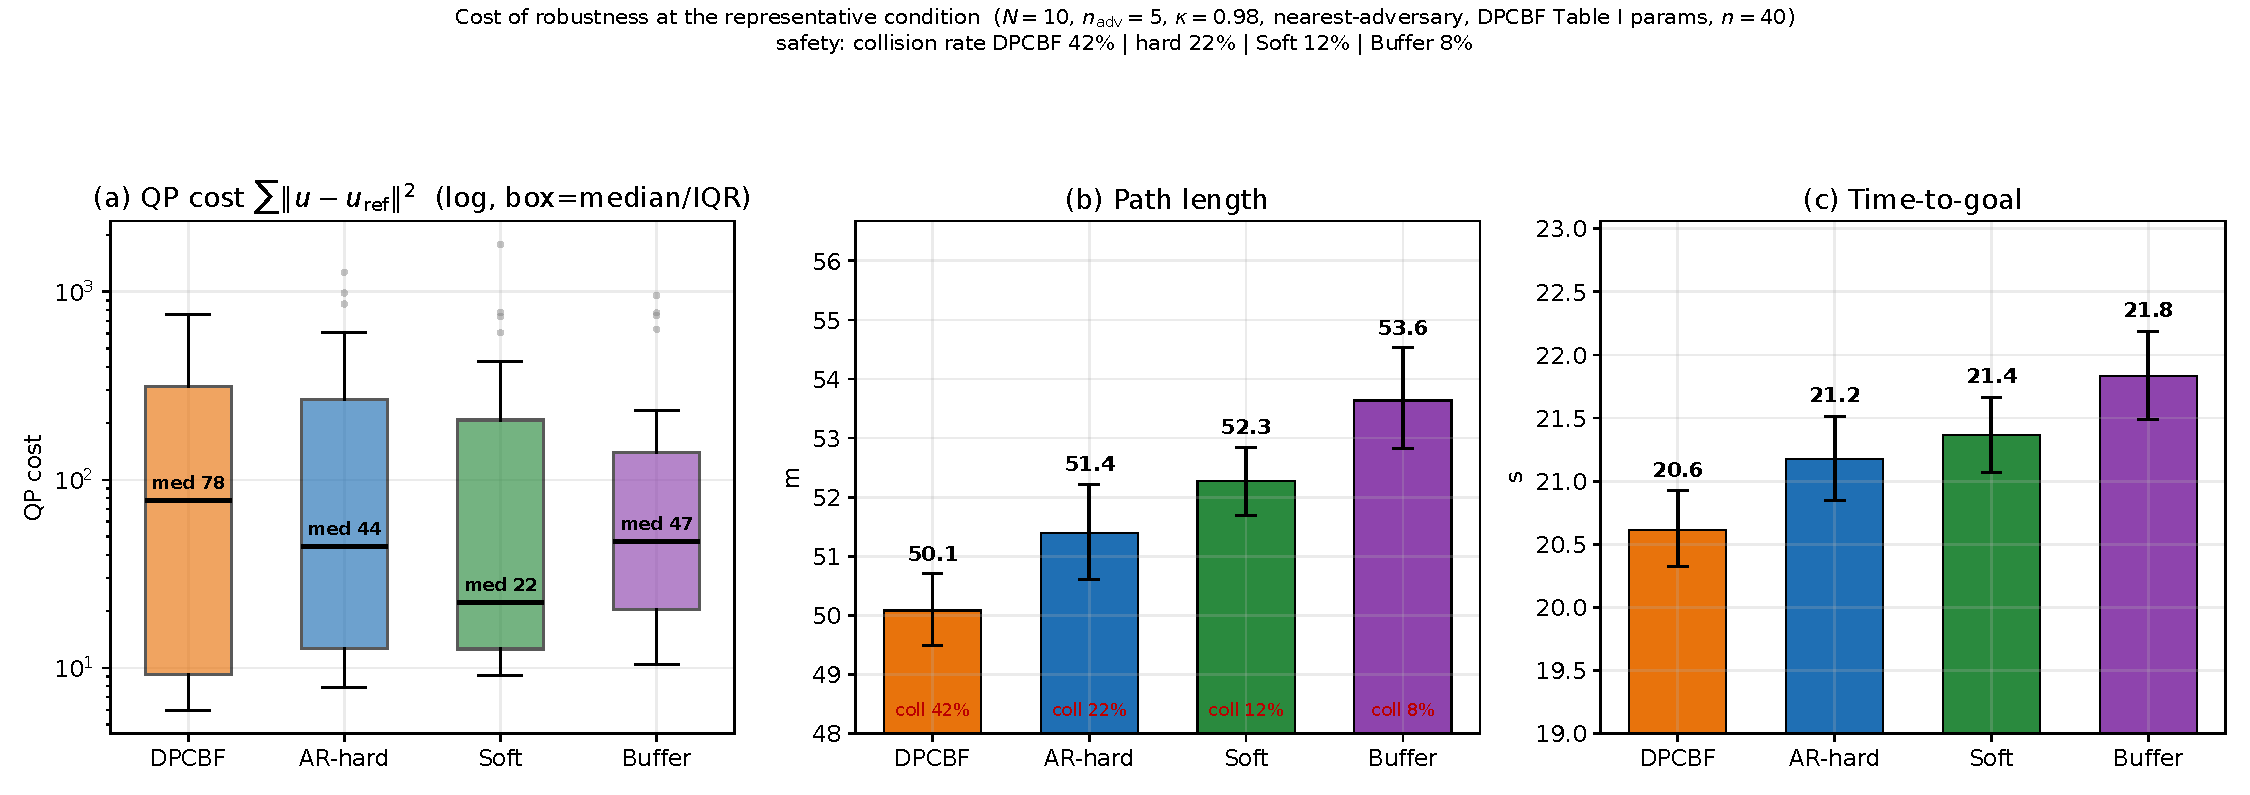
\includegraphics[width=\textwidth]{fig_cost.pdf}
  \caption{Cost of robustness at the representative condition
  ($N=10$, $n_{\mathrm{adv}}=5$). (a)~QP cost (median, log box plot);
  (b)~path length; (c)~time-to-goal, with collision rates annotated.
  Robustness costs a modest path/time detour but \emph{reduces} median
  control effort relative to the reactive baseline.}
  \label{fig:cost}
\end{figure*}

\paragraph{The pre-emption gain $\gamma$}
The gain $\gamma$ is the knob behind this trade-off: it interpolates between
reserving the full worst-case maneuver in the barrier parameters
($\gamma\!\to\!1$) and deferring entirely to the runtime margin of
Theorem~\ref{thm:validity} ($\gamma\!\to\!\infty$, where AR-DPCBF reduces to
DPCBF). Fig.~\ref{fig:gamma} ablates $\gamma\in[0.5,\infty)$ at $N=1$ and
$N=10$. For a single adversary every soft variant is violation-free for all
$\gamma$, matching the theory's exactness in the uncluttered regime. In the
multi-obstacle case the variants diverge: Soft's violation rate rises to
$76\%$ as $\gamma\!\to\!\infty$ (it inherits DPCBF's failure once no margin is
pre-reserved), whereas Buffer plateaus near $33\%$ because its proactive
buffer zone supplies robustness even without the parametric contraction. The
QP-infeasibility panel confirms both soft variants stay near zero for all
$\gamma$. We recommend the band $\gamma\in[1,3]$, which retains most of the
safety benefit without excessive conservatism.

\begin{figure*}[t]
  \centering
  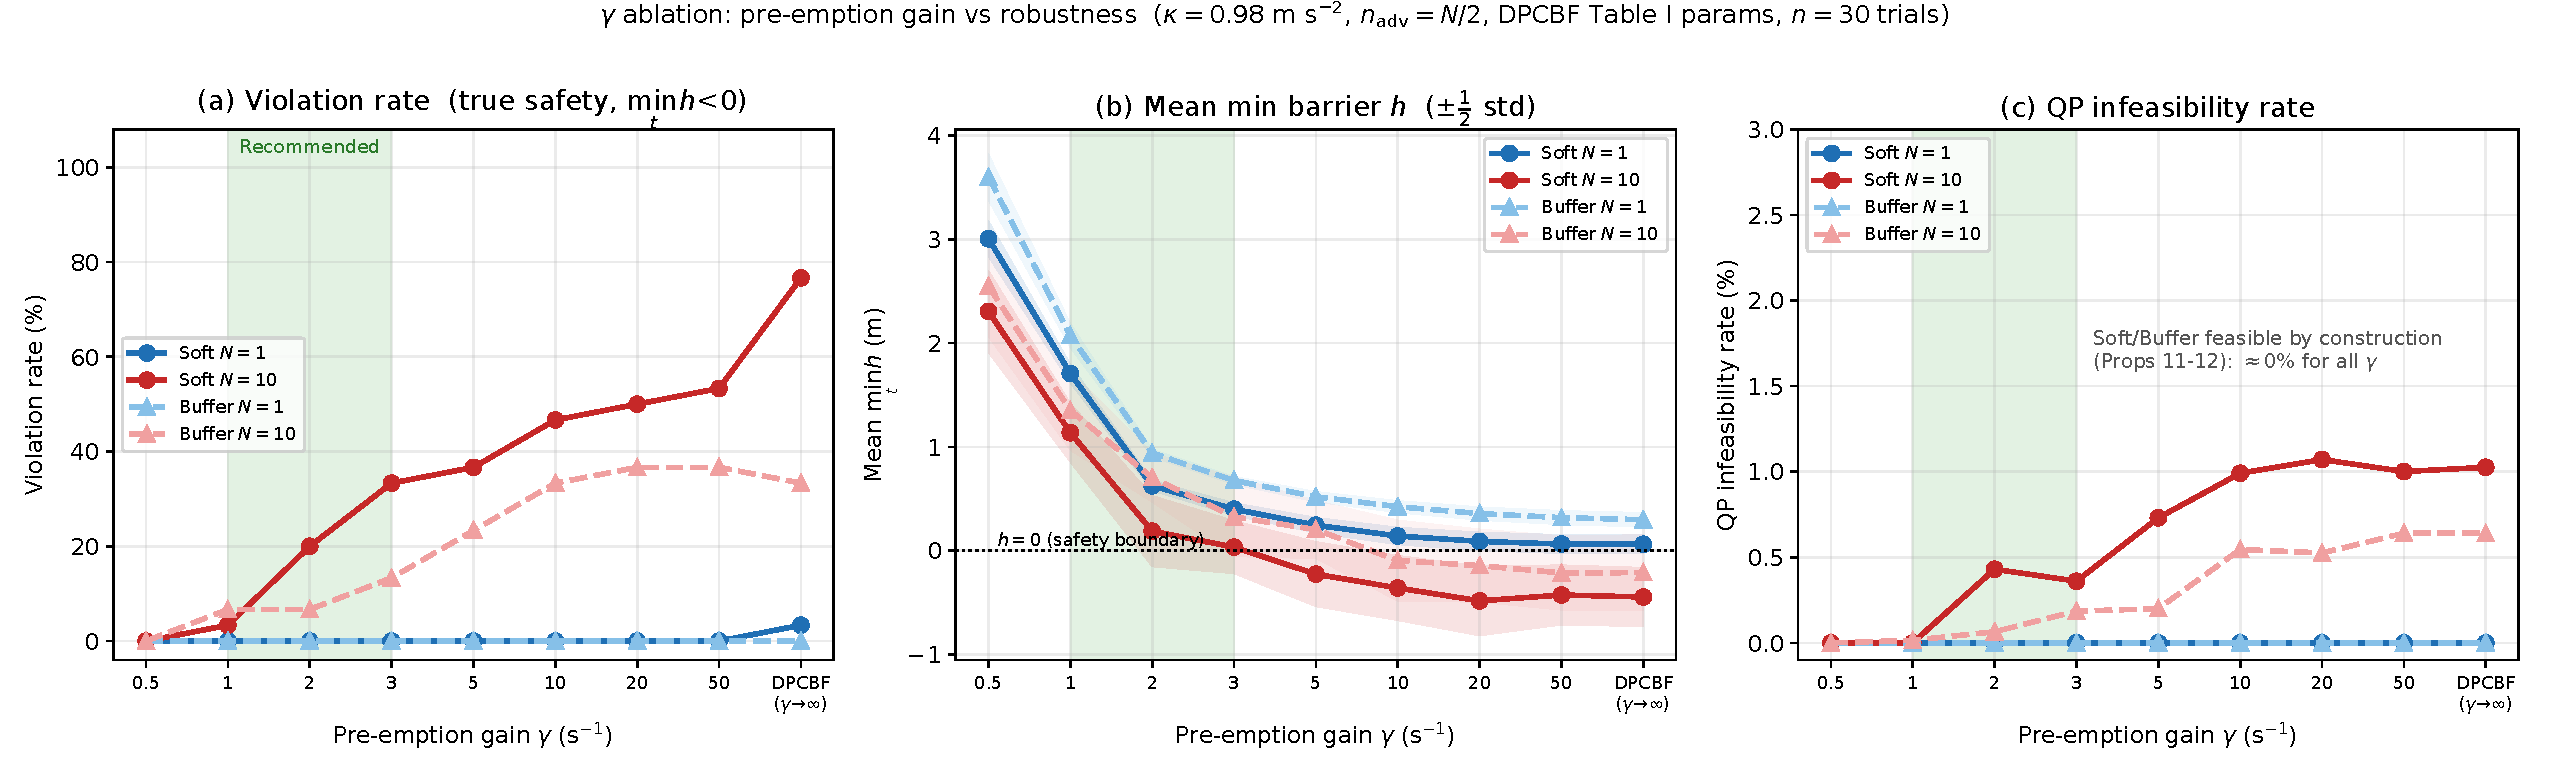
\includegraphics[width=\textwidth]{fig_gamma_ci_fix.pdf}
  \caption{Ablation of the pre-emption gain $\gamma$ ($n=30$). (a)~violation
  rate, (b)~mean minimum barrier, (c)~QP-infeasibility, at $N=1$ and $N=10$.
  $N=1$ is theory-exact for all $\gamma$; at $N=10$, Buffer plateaus while
  Soft degrades toward the DPCBF limit as $\gamma\!\to\!\infty$.}
  \label{fig:gamma}
\end{figure*}

% =====================================================================
\subsection{Validation of the Theoretical Guarantees}
\label{sec:theory}

The empirical behavior above is consistent with the paper's guarantees; we
now test those guarantees directly. We validate, in turn, the controllability
condition of the main theorem, the method's behavior when that condition is
violated by capability misspecification, and the online estimator that makes
the guarantee deployable.

\paragraph{Validity condition (Theorem~\ref{thm:validity})}
Theorem~\ref{thm:validity} guarantees that the adversarial certificate is
maintainable whenever the robot out-authorizes the obstacle,
$c_{\min}>\kappa$. We validate this by testing the underlying Nagumo
condition $\sup_{u\in U}\inf_{\mathcal F}\dot h^*\ge 0$ at sampled boundary
states $\{h^*=0\}$, with both authority channels limited to $c_{\min}$ and a
single matched adversary, so that the binding constraint is controllability
rather than multi-obstacle composition. Fig.~\ref{fig:boundary} maps the
fraction of boundary states at which the certificate is maintainable over the
$(\kappa,c_{\min})$ plane. The region certified by the theorem,
$c_{\min}>\kappa$ (above the dashed line), is uniformly safe: $100\%$ of
sampled boundary states admit a defending input, with no counterexamples. The
empirical failure cliff lies \emph{beyond} the line and the transition is
graceful rather than abrupt. The gap between the empirical cliff and
$c_{\min}=\kappa$ is expected: Theorem~\ref{thm:validity} bounds the
\emph{worst} boundary state through the infima $\Lambda_{\min}$, $D_{\min}$
and reserves only a $1/\gamma$ fraction of the maneuver, so the certified
line is a conservative envelope of the typical behavior. The figure thus
confirms the theorem as a sound, slightly conservative sufficient condition.

\begin{figure}[t]
  \centering
  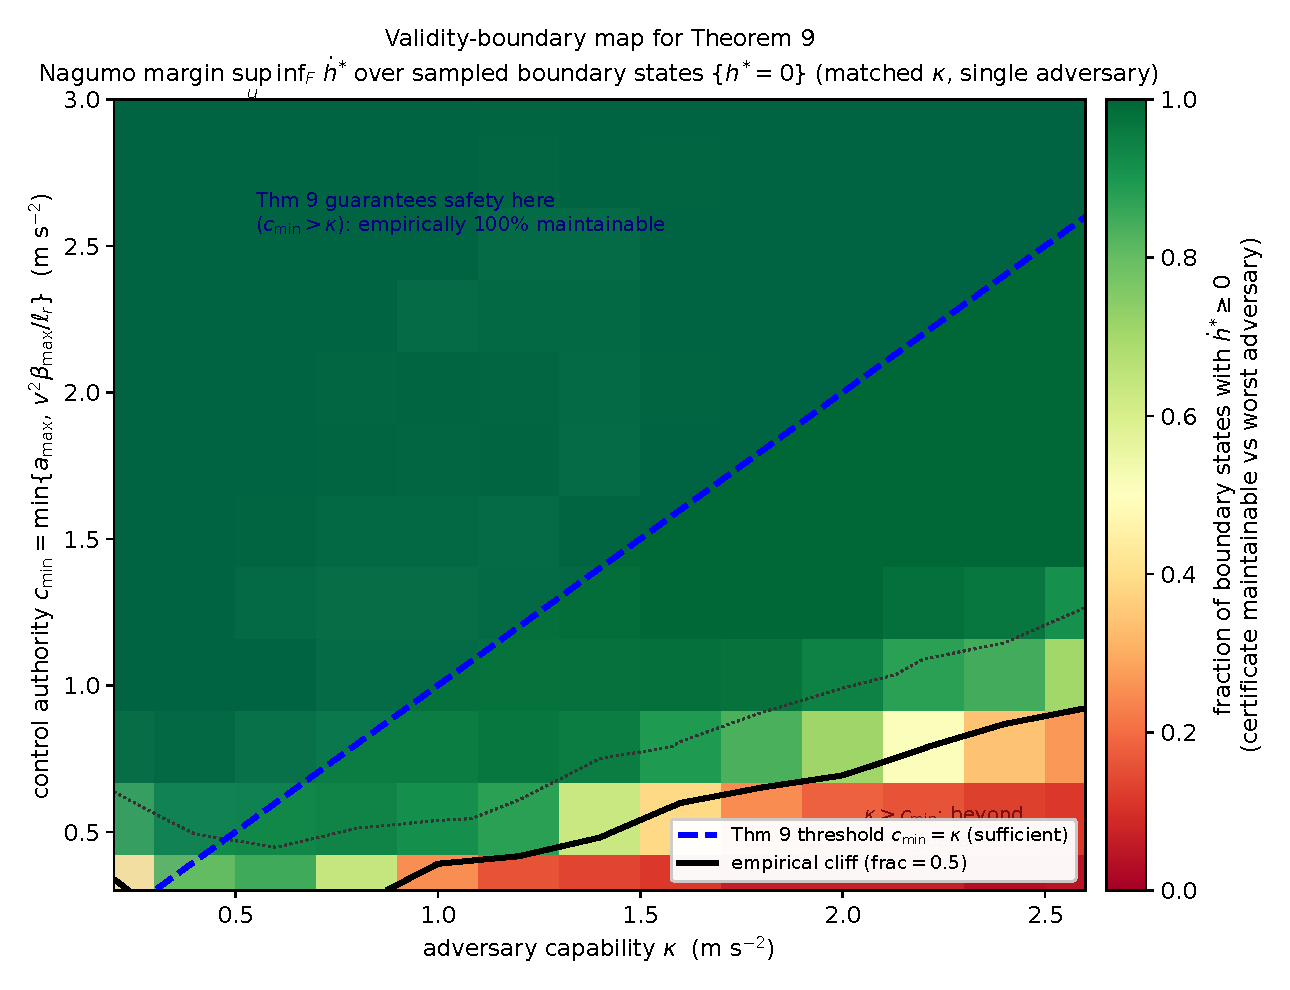
\includegraphics[width=\columnwidth]{fig_boundary.pdf}
  \caption{Validity-boundary map for Theorem~\ref{thm:validity}. Color is the
  fraction of boundary states $\{h^*=0\}$ where the worst-case Nagumo margin
  $\sup_u\inf_{\mathcal F}\dot h^*$ is non-negative. The certified region
  $c_{\min}>\kappa$ (above the dashed line) is uniformly maintainable; the
  empirical cliff lies beyond it.}
  \label{fig:boundary}
\end{figure}

\paragraph{Fail-safe under misspecification}
A safety-critical method must degrade gracefully when the obstacle is more
capable than assumed---that is, when the validity condition above is violated
in practice. Fig.~\ref{fig:misspec} holds the controller's assumed capability
fixed at $\kappa_{\mathrm{asm}}=0.98$ and sweeps the \emph{true} adversary
capability $\kappa_{\mathrm{true}}$ from $0.3$ to $2.0$. On the
over-provisioned side ($\kappa_{\mathrm{true}}<\kappa_{\mathrm{asm}}$) the
controller is conservative but safe, in fact \emph{safer} than a matched
controller (e.g. $13\%$ vs.\ $23\%$ violation at $\kappa_{\mathrm{true}}=0.7$),
since assuming excess capability simply enlarges the buffer. On the
under-provisioned side ($\kappa_{\mathrm{true}}>\kappa_{\mathrm{asm}}$)---the
dangerous case---the degradation is graceful and bounded: Buffer Soft
AR-DPCBF holds violations near $13\%$ and collisions near $6\%$ even when the
true capability is \emph{twice} the assumed value, never approaching the
$56$--$96\%$ violation of DPCBF. There is no cliff. We attribute the flatness
of the Buffer curve to its proactive Huber margin, which supplies spatial
robustness beyond the $\kappa$-dependent contraction; the Soft variant,
lacking this margin, degrades more (to $33\%$) though it too remains far below
the baseline. This is the principal evidence that AR-DPCBF---and Buffer in
particular---fails safe under capability uncertainty.

\begin{figure*}[t]
  \centering
  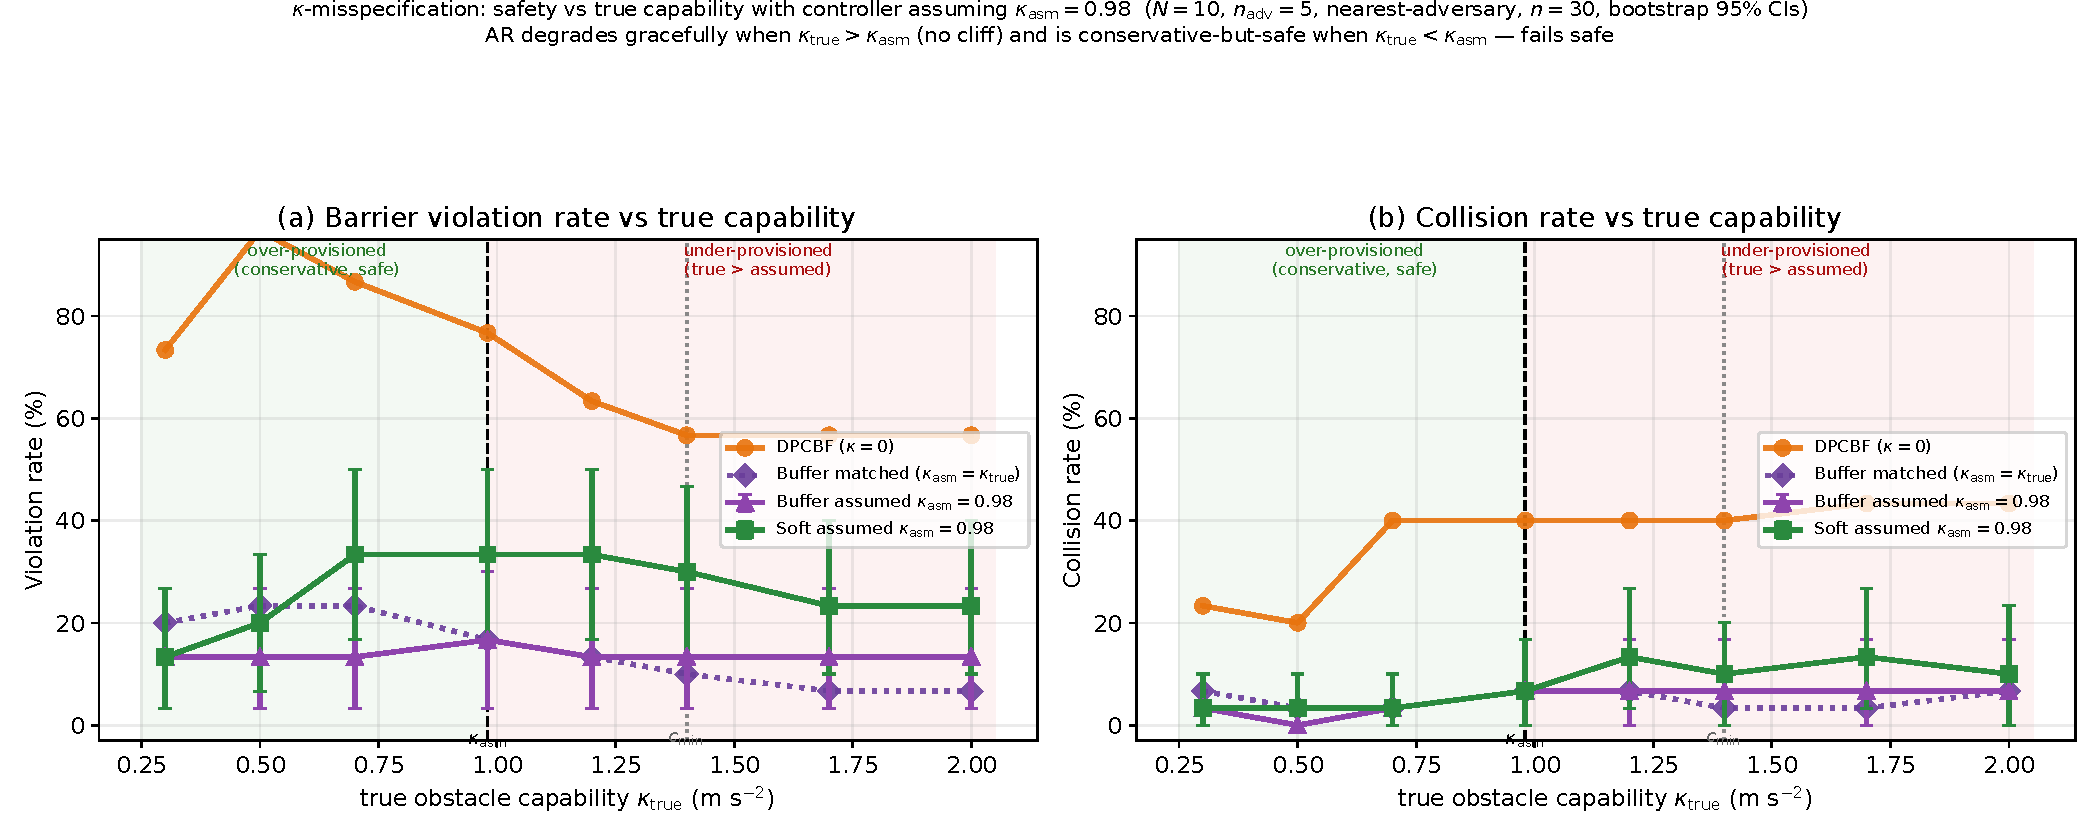
\includegraphics[width=\textwidth]{fig_misspec.pdf}
  \caption{$\kappa$-misspecification: safety versus true capability with the
  controller assuming $\kappa_{\mathrm{asm}}=0.98$ ($n=30$). (a)~violation,
  (b)~collision. AR degrades gracefully (no cliff) when
  $\kappa_{\mathrm{true}}>\kappa_{\mathrm{asm}}$ and is conservative-but-safe
  when $\kappa_{\mathrm{true}}<\kappa_{\mathrm{asm}}$.}
  \label{fig:misspec}
\end{figure*}

\paragraph{Closed-loop operation with the online estimator}
The two validations above assume $\kappa$ is known. In practice it is
estimated online by the sliding-window estimator of
Section~\ref{sec:estimation}, whose coverage guarantee is
Proposition~\ref{prop:est}. Fig.~\ref{fig:closedloop} closes this loop: each
adversary's capability is estimated per-cycle from noisy $(v,\theta)$
measurements and fed back into the controller, and we compare the resulting
safety to an oracle that knows $\kappa$ exactly. The estimated-capability
controller is \emph{at least as safe as} the oracle at every noise level
(violation $\le 33\%$, collision $\le 10\%$, versus DPCBF's $77\%/27\%$), and
is in fact strictly safer because the sub-Gaussian margins make the estimate
dominate the truth: the empirical coverage $P[\tilde\kappa\ge\kappa]$ is
$0.96$--$1.00$ and the mean estimated capability grows with sensor noise
($1.45\!\to\!11.5$ as $\sigma_v$ goes from $0.02$ to $0.20$). As
$\sigma_v\!\to\!0$ the margins vanish and the estimator converges to the
oracle. This is exactly the behavior Proposition~\ref{prop:est} predicts:
monotonicity of $(\lambda^*,\mu^*)$ in $\kappa$ (Theorem~\ref{thm:params}(i))
turns over-coverage of $\kappa$ into a more conservative, hence safe,
controller. The price of the noise-induced over-coverage is conservatism, not
safety.

\begin{figure*}[t]
  \centering
  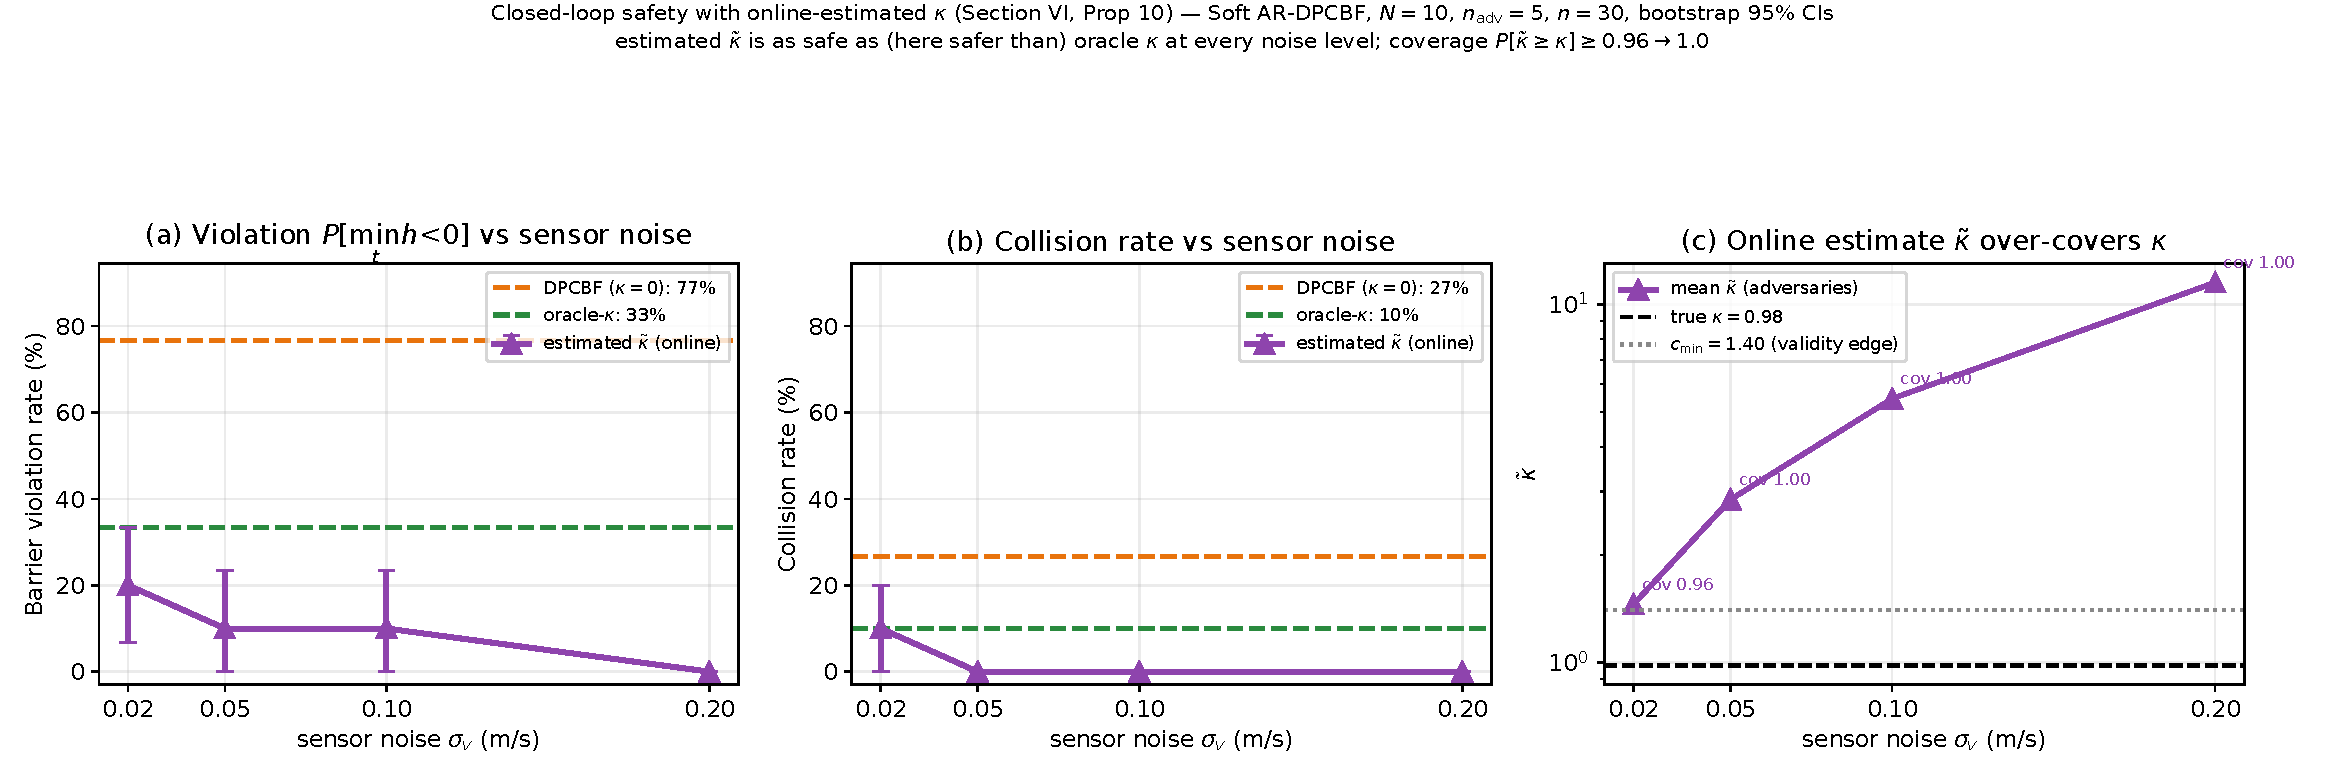
\includegraphics[width=\textwidth]{fig_closedloop.pdf}
  \caption{Closed-loop safety with the online-estimated capability
  (Section~\ref{sec:estimation}, Proposition~\ref{prop:est}; Soft AR-DPCBF,
  $n=30$). (a)~violation and (b)~collision versus sensor noise, with DPCBF and
  oracle-$\kappa$ as references; (c)~the estimate $\tilde\kappa$ over-covers
  the true $\kappa$ with coverage $P[\tilde\kappa\ge\kappa]\ge 0.96$.}
  \label{fig:closedloop}
\end{figure*}

% =====================================================================
\subsection{Summary}
\label{sec:summary}

The study supports every structural claim of the paper, and the figures build
a single argument. The silent-failure mode of Remark~\ref{rem:gap} is real and
severe ($95\%$ violation, $60\%$ collision for DPCBF under a dense maneuvering
population) and is removed by all AR variants, with the ordering
$\text{Buffer}<\text{Soft}<\text{Hard}<\text{DPCBF}$ in violation depth
(Fig.~\ref{fig:adv}), at pooled significance $p<10^{-3}$
(Fig.~\ref{fig:mcnemar}). The result is general across both axes of the
threat space: it holds for every adversary capability with exact recovery at
$\kappa=0$ (Fig.~\ref{fig:cap}), and it scales with density, where the soft
variants preserve QP feasibility that Hard AR loses
(Fig.~\ref{fig:density}, Propositions~\ref{prop:soft}--\ref{prop:buffer}).
This robustness costs only a $\sim\!7\%$ path detour and \emph{reduces}
control effort (Fig.~\ref{fig:cost}), tunable through the single gain $\gamma$
(Fig.~\ref{fig:gamma}). Finally, the theory is confirmed directly: the
validity condition of Theorem~\ref{thm:validity} holds with no counterexamples
(Fig.~\ref{fig:boundary}), the method fails safe under capability
misspecification (Fig.~\ref{fig:misspec}), and the online estimator preserves
safety in closed loop (Fig.~\ref{fig:closedloop},
Proposition~\ref{prop:est}). Across the board, Buffer Soft AR-DPCBF is the
recommended controller: it is the only variant significant against both
baselines on both safety axes, it tolerates a misspecified capability, and it
retains feasibility and efficiency.

\end{document}
